\subsection{Diving into the Complexity}

Now that the scale of the scanned code base, what does the \cc of that code base look like?

\begin{figure}
	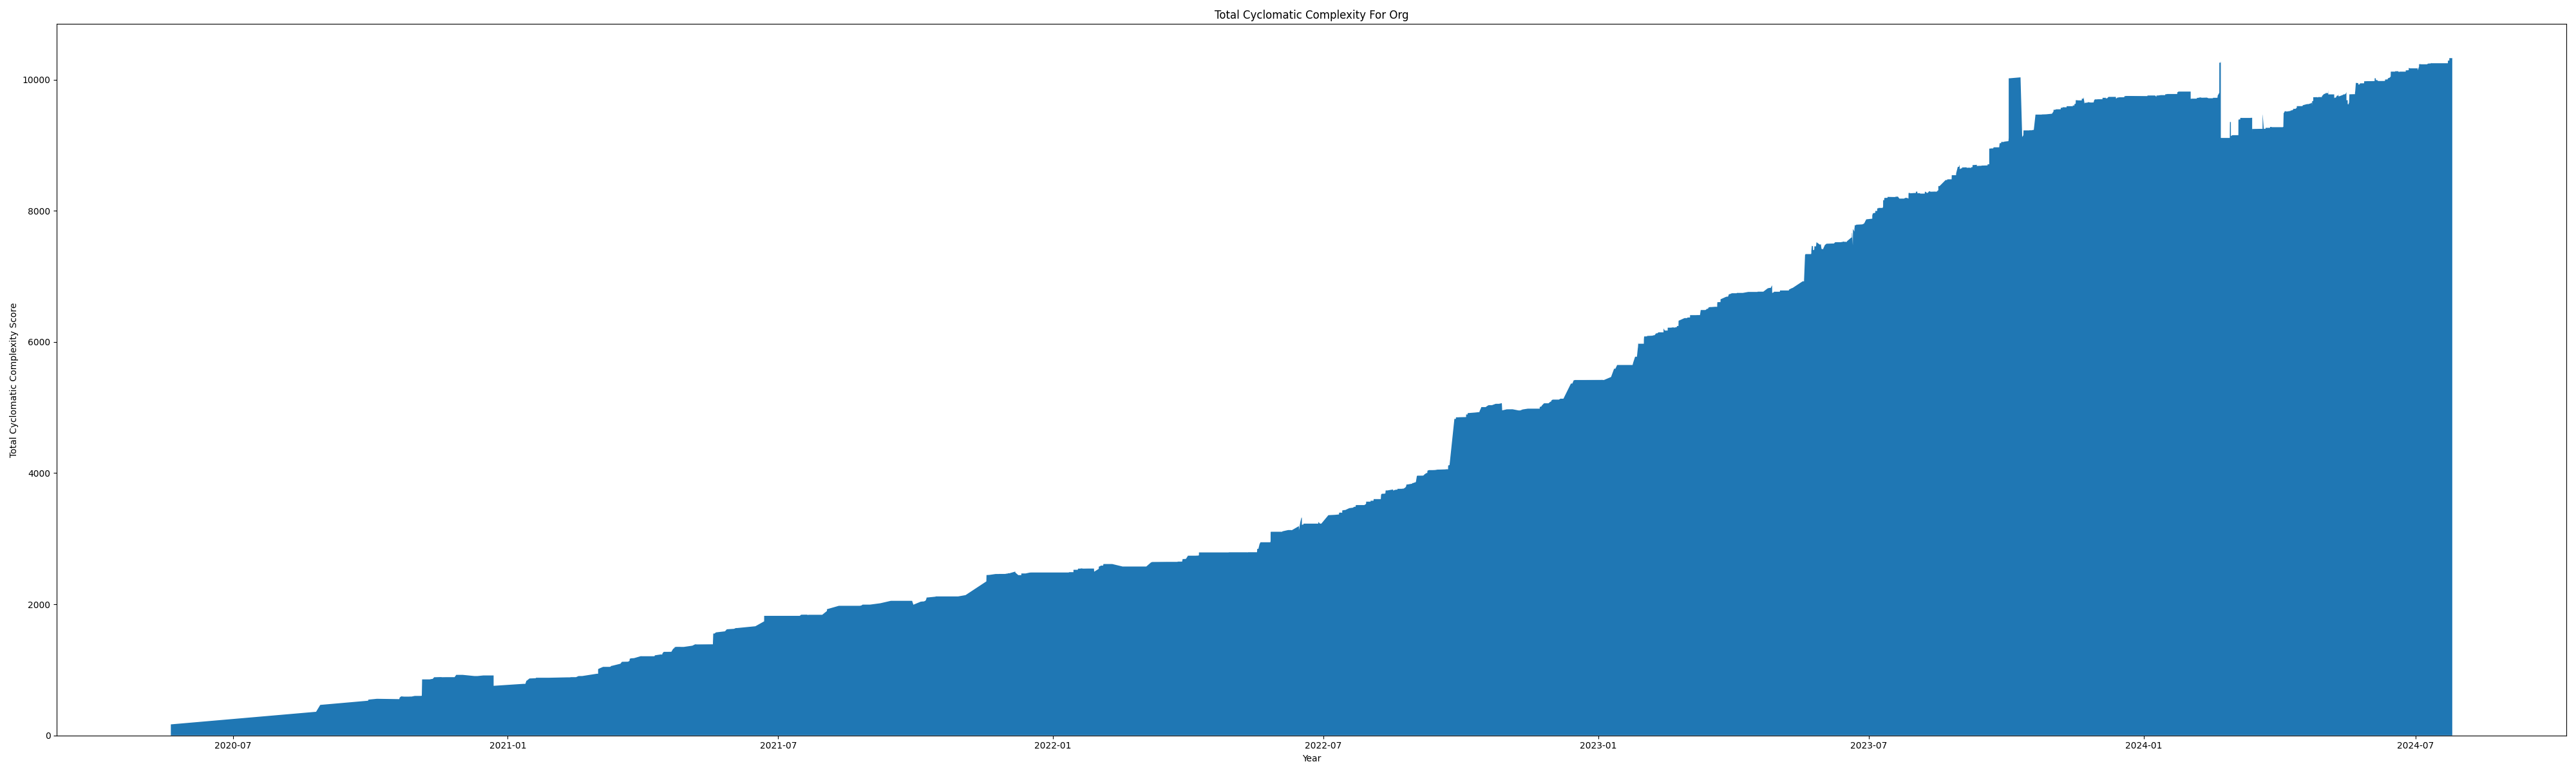
\includegraphics[width=\textwidth]{project_cc.png}
	\caption{\cc for the source code}
	\label{fig:project_cc}
\end{figure}

In \textbf{Figure \ref{fig:project_cc}} the \cc is scored overtime.
The main takeaway from this is how the project as a whole is nearly doubling in complexity every year.
A new user joining the project a year ago would have found it much easier to onboard.
When the data is ranked, it shows a different picture.

\begin{figure}
	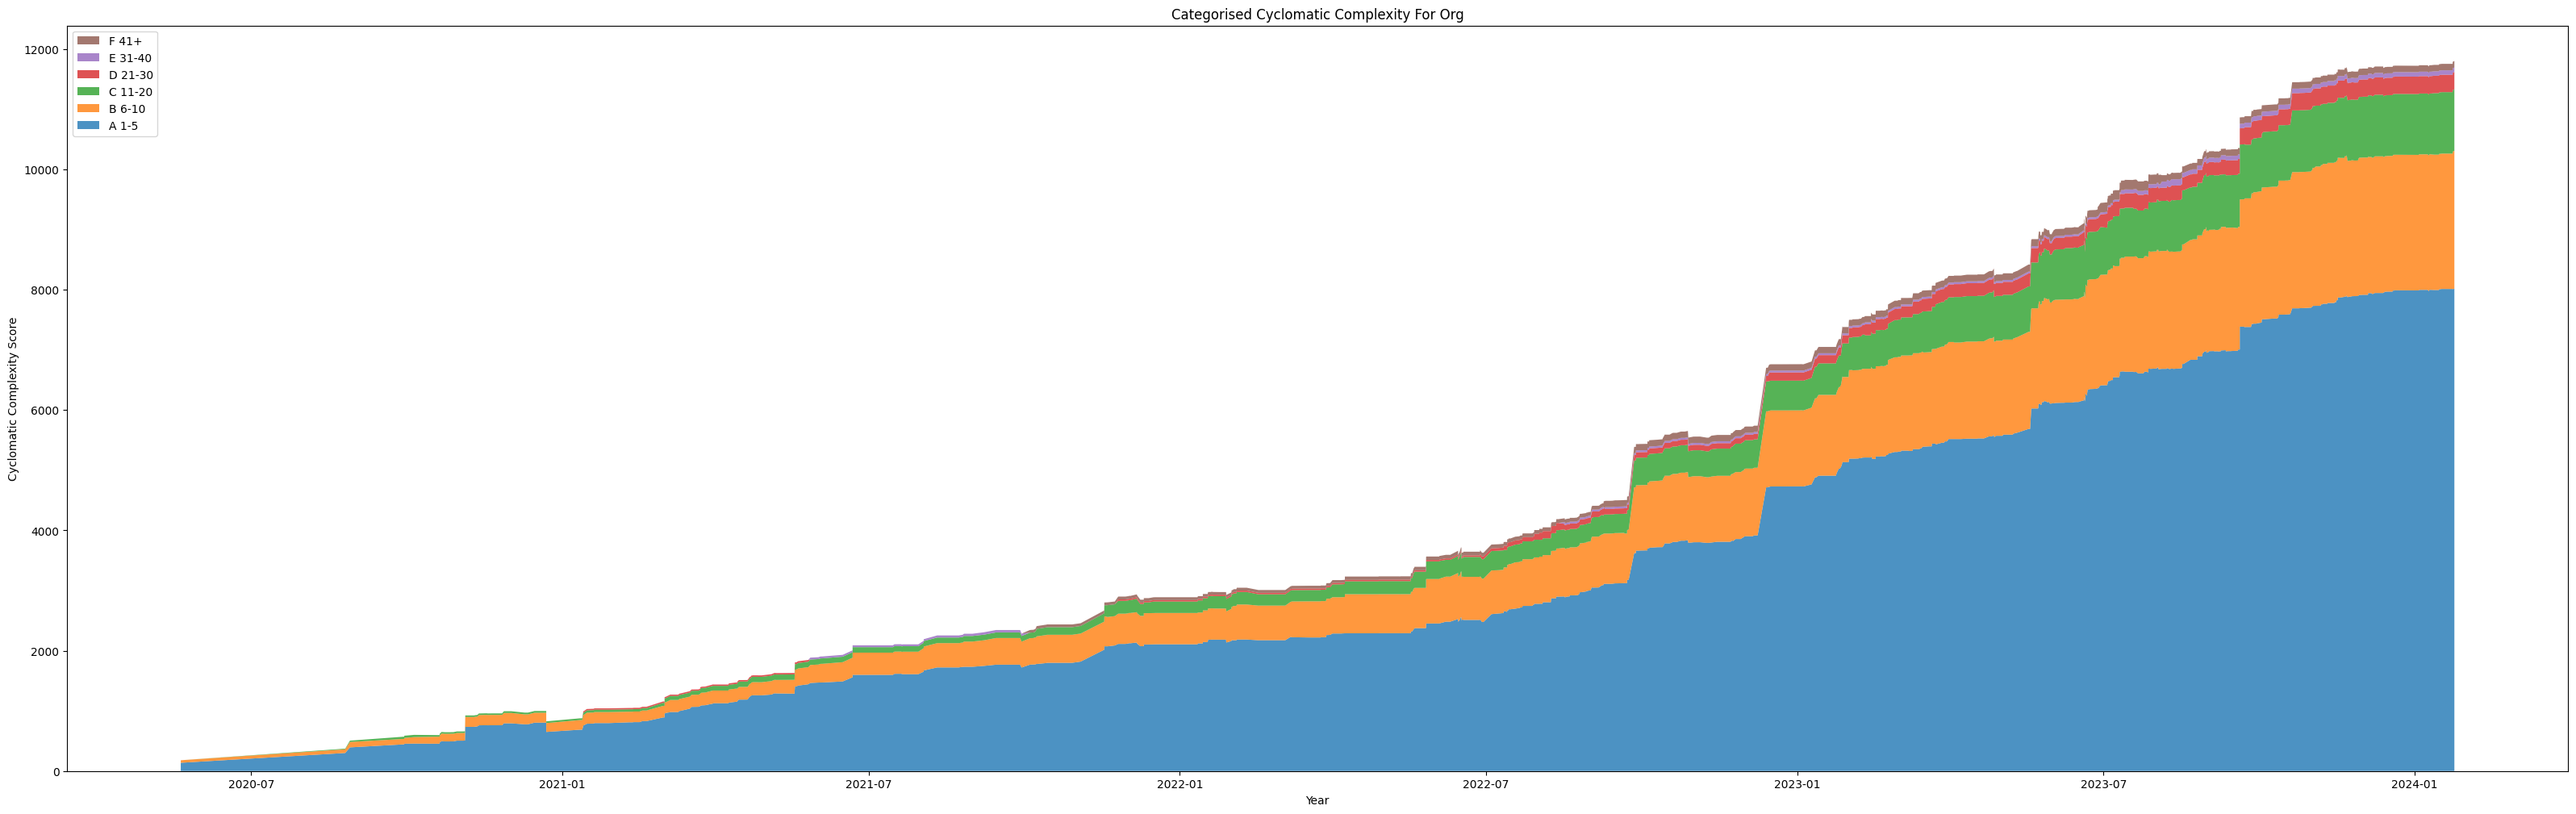
\includegraphics[width=\textwidth]{project_group_cc.png}
	\caption{\cc score ranked}
	\label{fig:project_group_cc}
\end{figure}

In \textbf{Figure \ref{fig:project_group_cc}}, by far the largest Rank is the A group which is at least two thirds the overall score.
Over the history of the project, this has always been the largest group.
For new users, this means most functions are simpler to understand the logic, but it does mean there are a lot more interfaces / functions that need to be learned.

\begin{figure}
	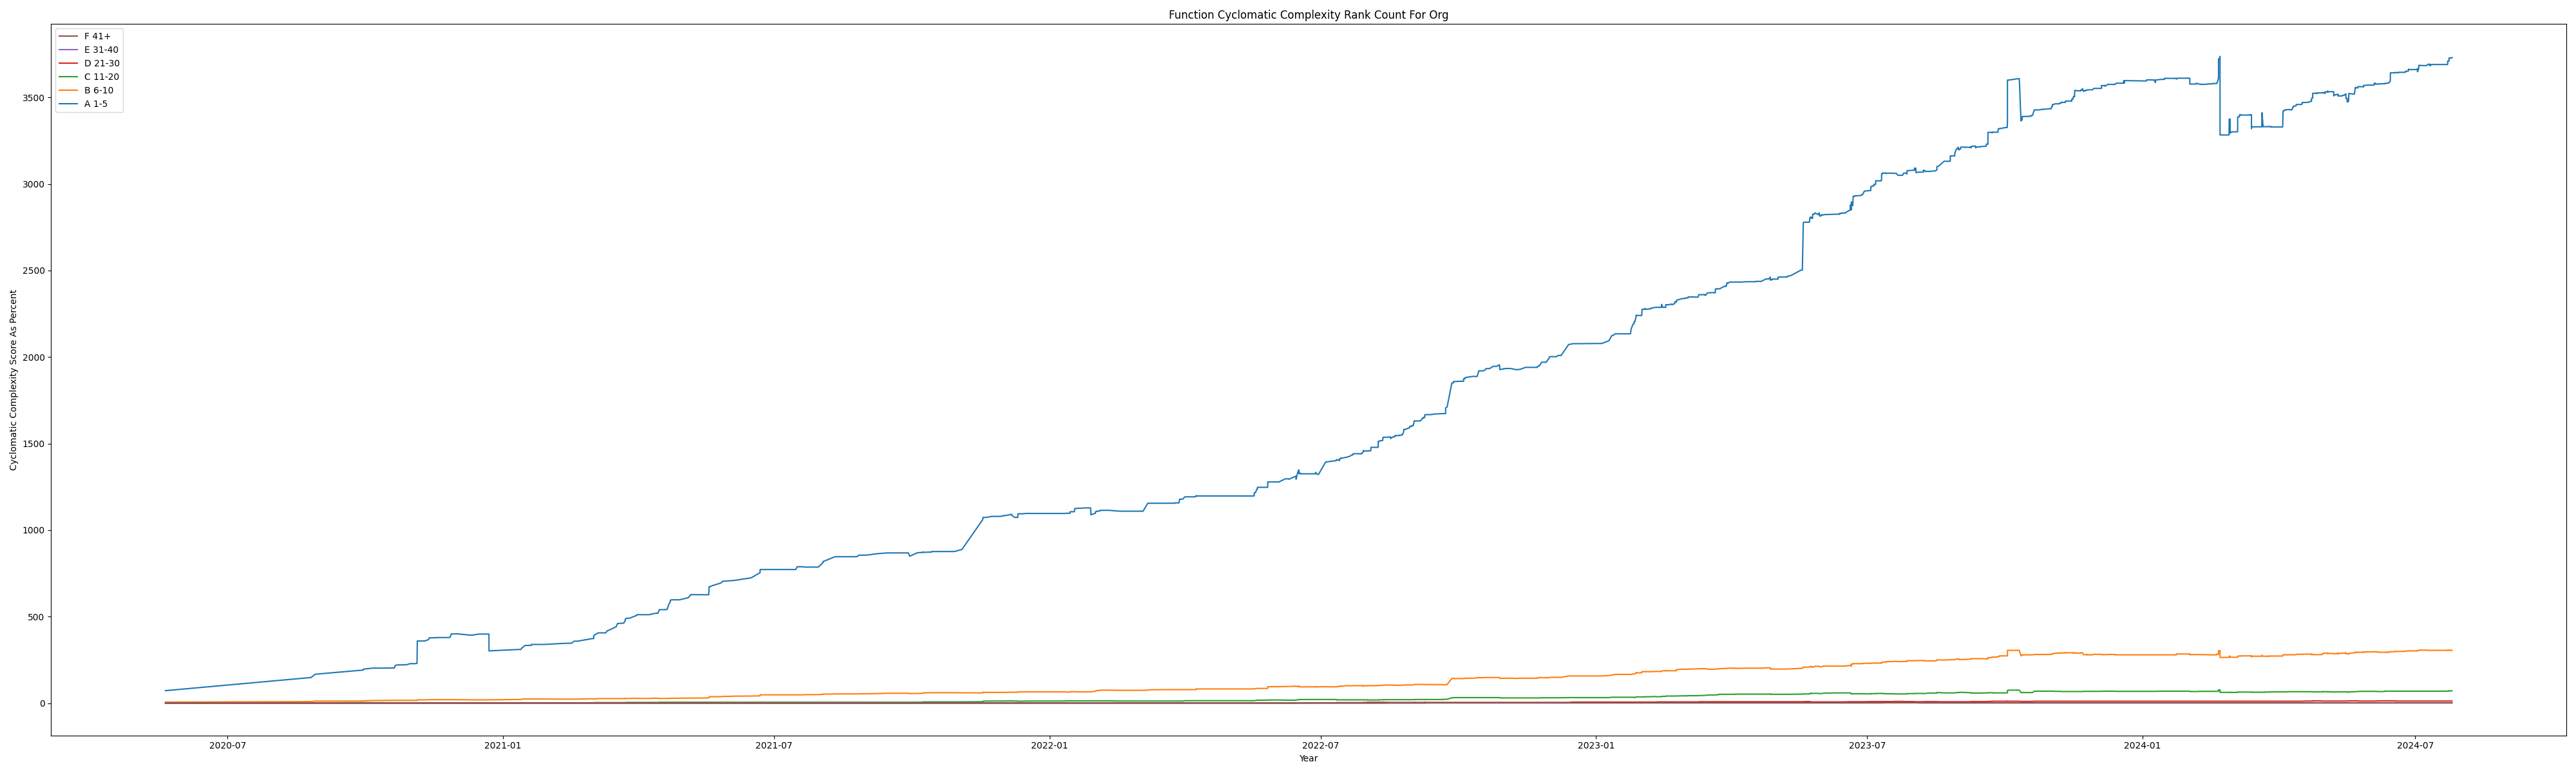
\includegraphics[width=\textwidth]{project_function_count_chart.png}
	\caption{Count of functions in each Rank for the Kuadrant Project}
	\label{fig:project_function_count_chart}
\end{figure}

Forgetting about \cc as a sum but looking at the number of functions in each Ranking, we see how different the scale between each rank.
In \textbf{Figure \ref{fig:project_function_count_chart}} the number of Rank A functions out scales all other ranks.
New users would be required to understand how these Rank A function's tide together.

Only two components in the Kuadrant project have the Rank A grouping less than 50\% of the overall ranking (authorino-operator, multicluster-gateway-controller).
Other components have some other interesting aspects that well be covered.
Not all graphs for each component will be covered here, as there are too many and the data will be out of date quickly.
For that reason, the notebooks that generate all the charts are located \href{https://www.github.com/Boomatang/cyclomatic-complexity}{here}.
% TODO get the notebook into a container to be run by others.

\subsubsection{The wasam shim project}
The wasam shim shows a nice outcome from looking at the \ccnsp, it shows how the project evolved over time.
In \textbf{Figure \ref{fig:total_cc_wasam_shim}} shows how the project grows in complexity over time but also that it can be refactored.
For some time, there were Rank E functions in the code base, which possibly replaced some Rank D functions.
However, now all the Rank E and D functions have been written out, but the over all \cc has not changed much.

A project's complexity will increase over time, and the Ranking of that complexity can also increase, but does not mean it cannot be refactored out at a later date.
This would also point to adding CI checks to ensure the \cc is kept below some arbitrary number might harm productivity within the project over time.

The pattern of refactoring out these complex functions from different Rankings can be seen in other components, but the wasam shim has the cleanest graph for showing this.
While it might be hard, we can make changes to refactor the API without changing the overall complexity of the component.
\begin{figure}
	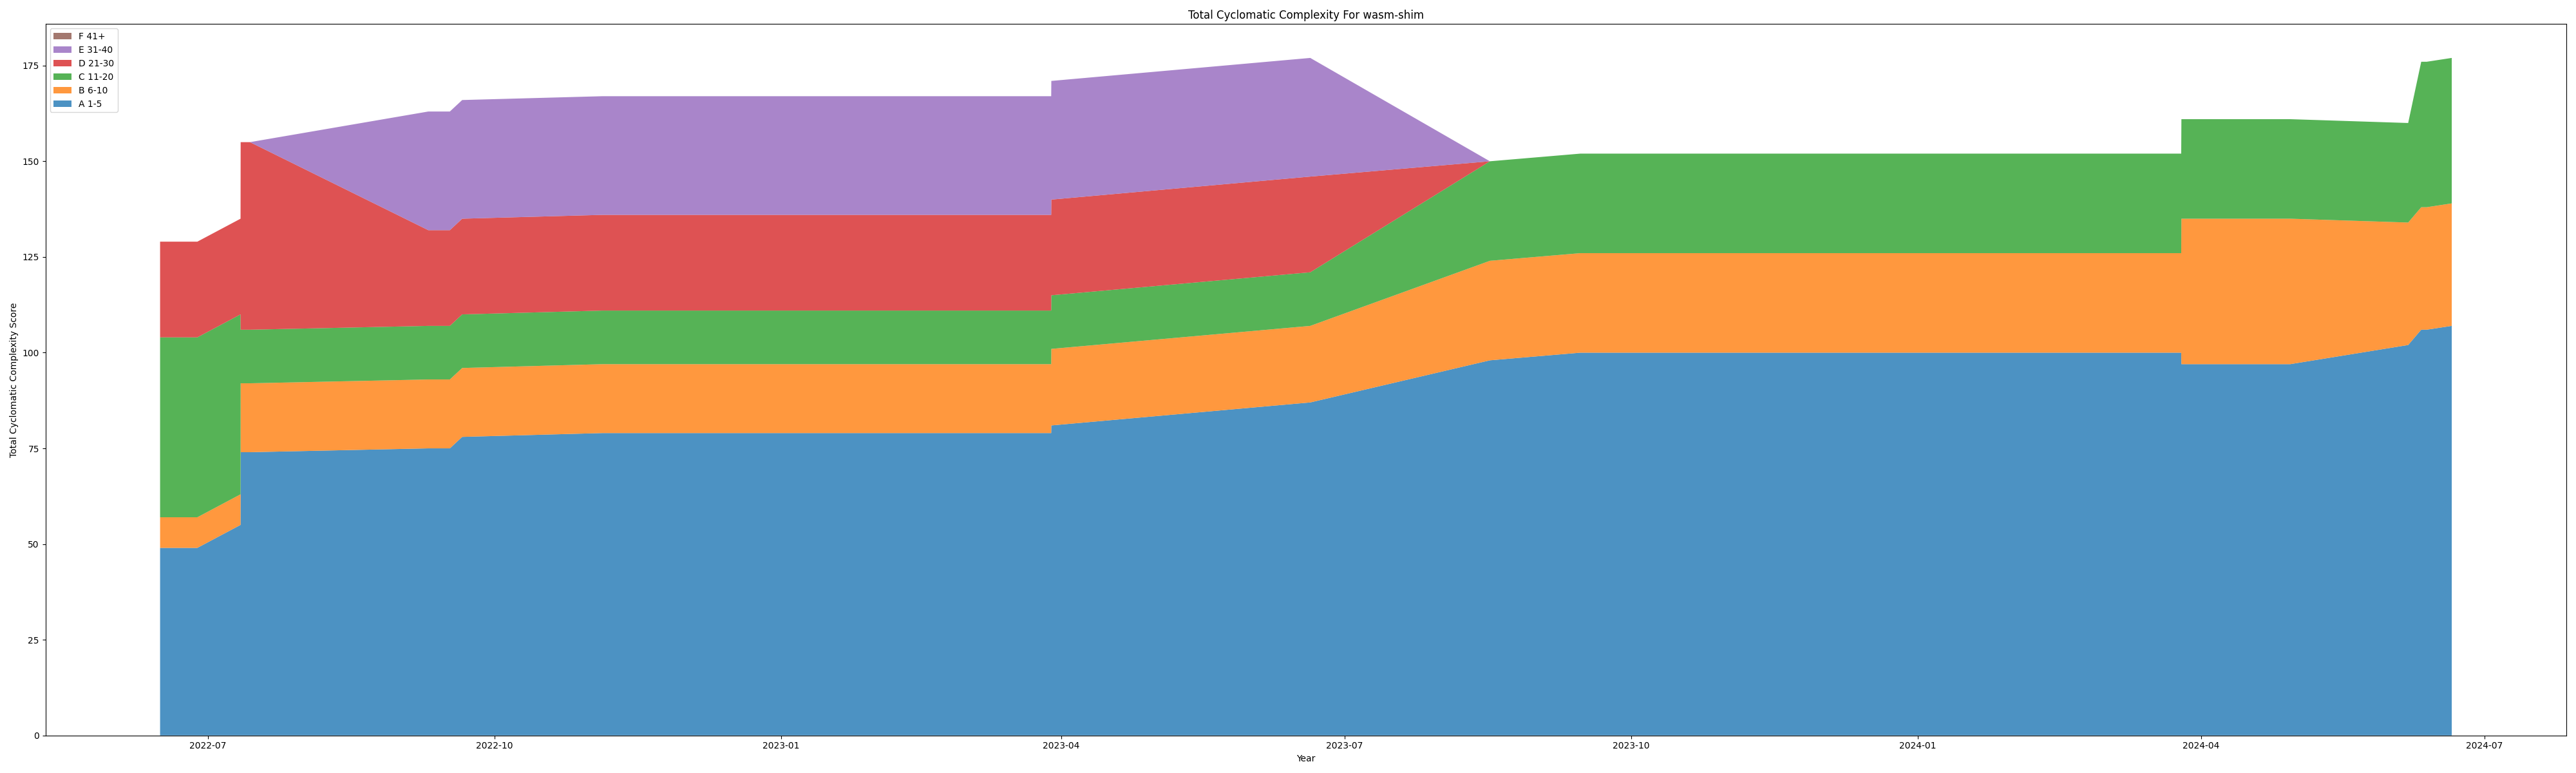
\includegraphics[width=\textwidth]{total_cc_wasm_shim.png}
	\caption{Total \cc over time for the wasam shim}
	\label{fig:total_cc_wasam_shim}
\end{figure}

\subsubsection{The limitador project}
Limitador was one of the projects that were going to be interesting as it is written in Rust, and one of the assumptions made was about Rust.
This showed a very surprising turn around, one that I was not expecting.
As a reminder, the assumption was Rust code because of its compile checks and language features would lead to functions that naturally would have a lower \cc score.

However, that is not the case.
In \textbf{Figure \ref{fig:total_cc_limitador}} the Ranking of the \cc changed over time, going to from lower Ranks to higher Ranks.
Around July 2022 there was a change to the project, and this change showed an increase in the \cc.
This was the joining of new members to the project.
New members can have their own views on what complexity can and should be.
If there is a belief in deep interfaces over wide interfaces, the \cc score will naturally be higher.

This shows that the \cc is as much affected by team culture and design philosophy as language features and project complexity.

\begin{figure}
	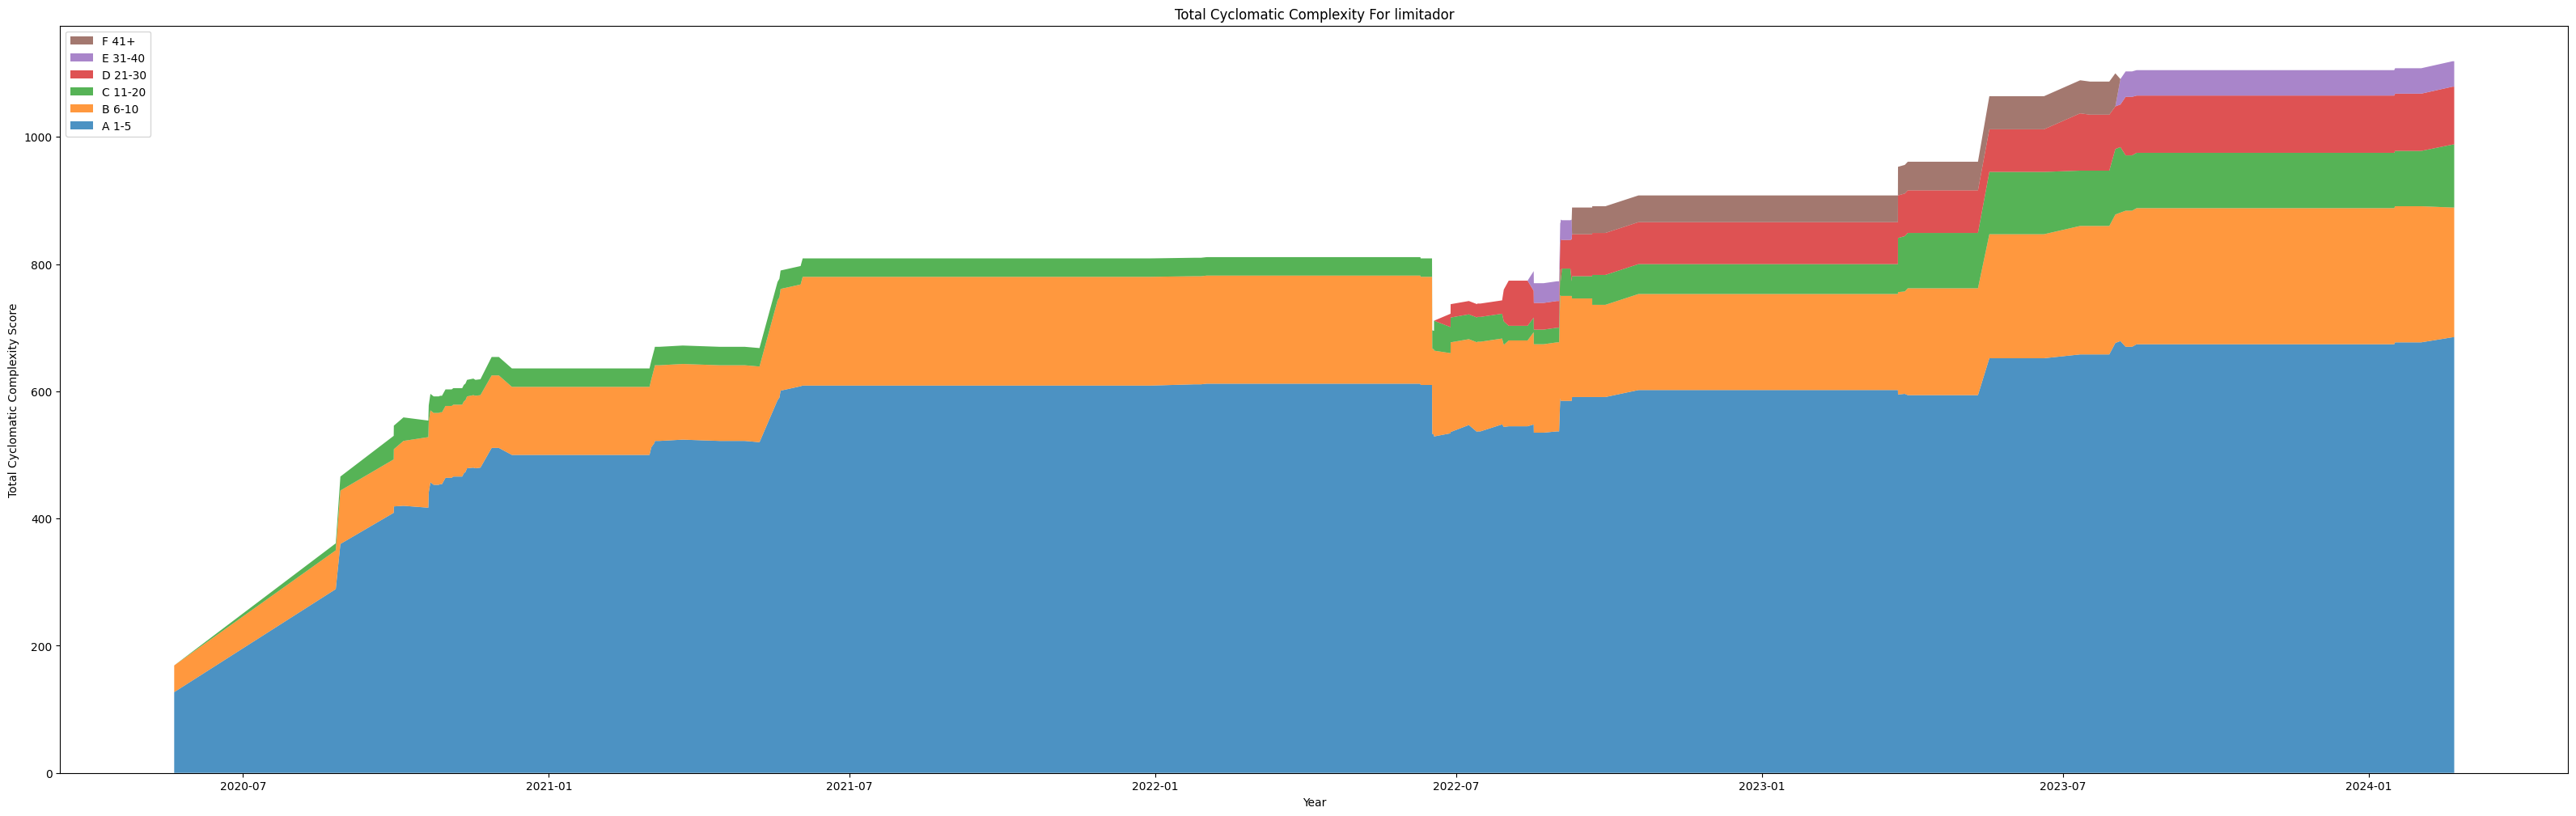
\includegraphics[width=\textwidth]{total_cc_limitador.png}
	\caption{Total \cc over time for limitador}
	\label{fig:total_cc_limitador}
\end{figure}

\subsubsection{The testsuite repo}
The testsuite repo was always going to be an interesting component of the Kuadrant project.
It can't be called a component as it is never shipped to the user, it is our test suite for our shipped components.
There is also the fact it is not written by the core engineering team but quality engineering, who are always understaffed and has other focus.
The other outlier is the repo is written in Python.
Python falls into the language assumption that \cc of functions would be less as Python duck typing allows the writing to get away with avoiding complexity.

What was not expected was the shear scale of the difference between the testsuite repo and every other repo in the Kuadrant project.
\textbf{Figure \ref{fig:total_cc_testsuite}} shows the scale of the differences.
Nearly 90\% of all functions are in the Rank A grouping.
This difference is so large that I wanted to know what the breakdown of the Rank A function.
The current state of the repo can be seen in the pie chart, \textbf{Figure \ref{fig:testsuite_pie_chart}}.

While this does align with the assumption made in the start, but seeing these numbers raised a concern for me.
How do new developers understand this repo?
Hopefully, the documentation for the repo explains how to combine all the functions to get the required result.

But is there more going on here?
This is a testsuite that uses pytest to run all the tests, so it is not being run by Python in the normal sense.
In pytest the \textit{assert} keyword is used to create any checks, which should not be used in production Python.
The \textit{assert} keyword can be disabled when using Python directly, this may mean the tool for calculating the \cc does not count the \textit{assert} keyword, and the project is far more complex than expected.
This was very much the case.
Looking at some of the near 500 functions that have a \cc score of 1, a lot have many \textit{assert} keywords with in the one function.
The \cc for the whole project is much higher than the tooling is leading us to believe, and not just that some functions are underreported.

\begin{figure}
	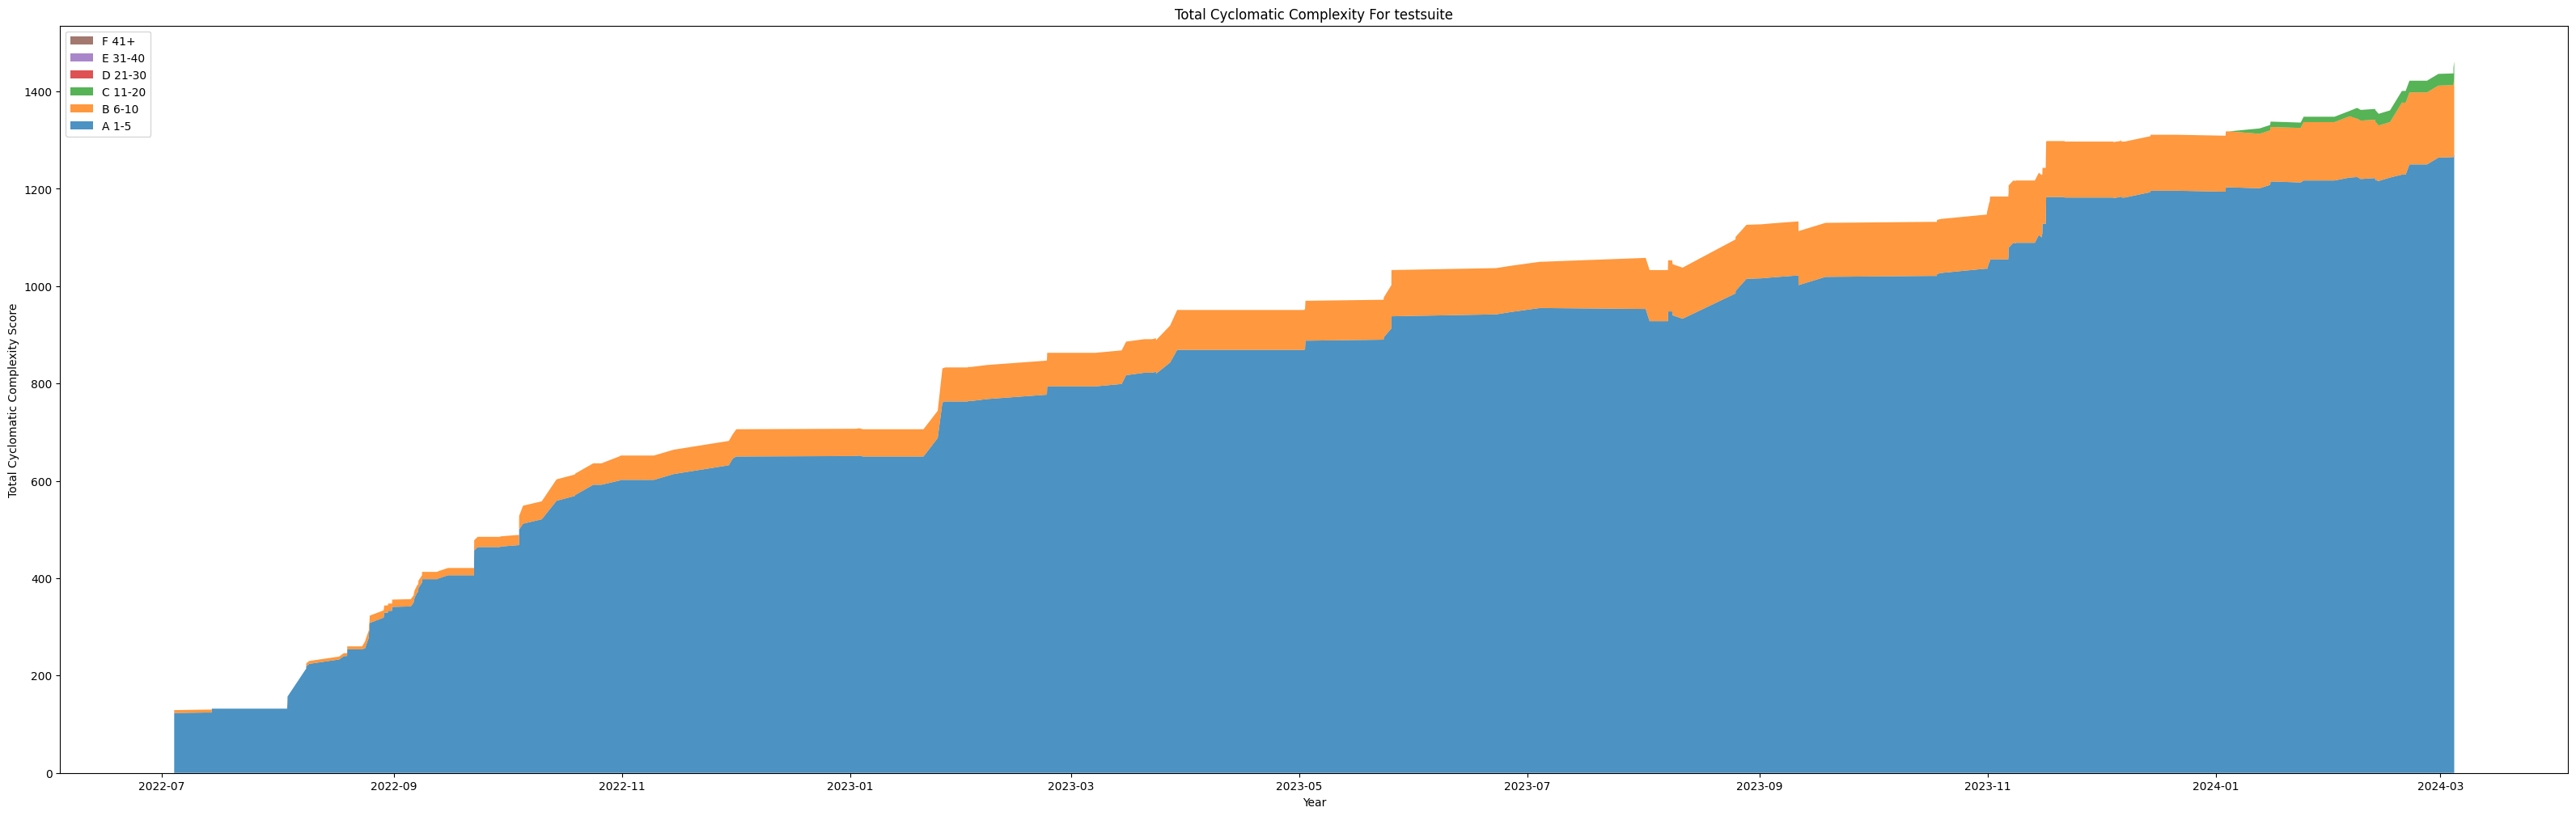
\includegraphics[width=\textwidth]{total_cc_testsuite.png}
	\caption{Total \cc over time for testsuite.}
	\label{fig:total_cc_testsuite}
\end{figure}

\begin{figure}
	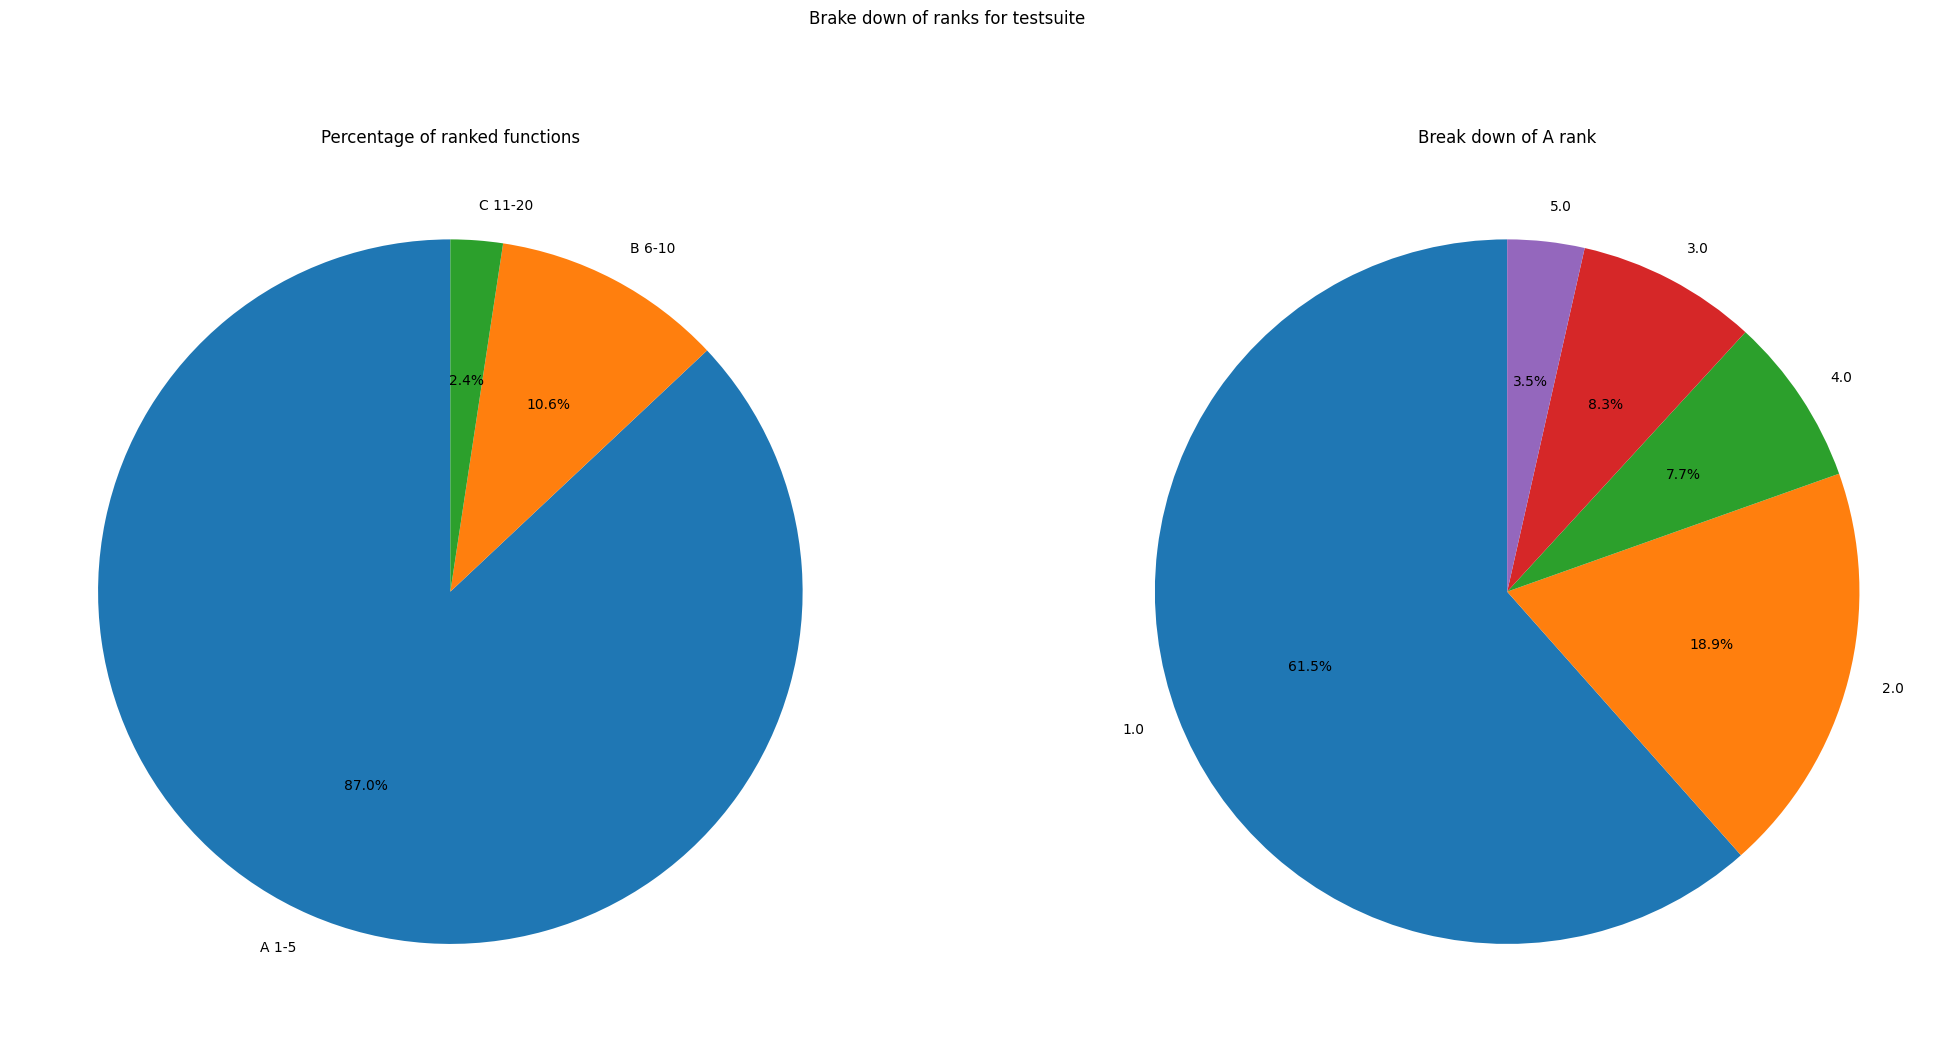
\includegraphics[width=\textwidth]{testsuite_pie_chart.png}
	\caption{Pie chart of testsuite rankings.}
	\label{fig:testsuite_pie_chart}
\end{figure}

\subsubsection{The multicluster-gateway-controller project}
Looking at the history of a project can revel change over time.
Apart from the normal growth of a project, historical events can be detected.
This can be events where features were added or removed.
These events normally show as jumps in the graphs over being a spike in the graph.

No project shows a better example of this than the multicluster-gateway-controller, as seen in \textbf{Figure \ref{fig:total_cc_mgc}}.
This relates to the removal of the DNS and TLS controllers from the project.
While these features are being refactored into the kuadrant-operator, it is still nice to see such changes.
In this case, it was a massive removal change that is easy to spot.
In very project, you can see a number of spikes that would be the result of new features being added to a project.

\begin{figure}
	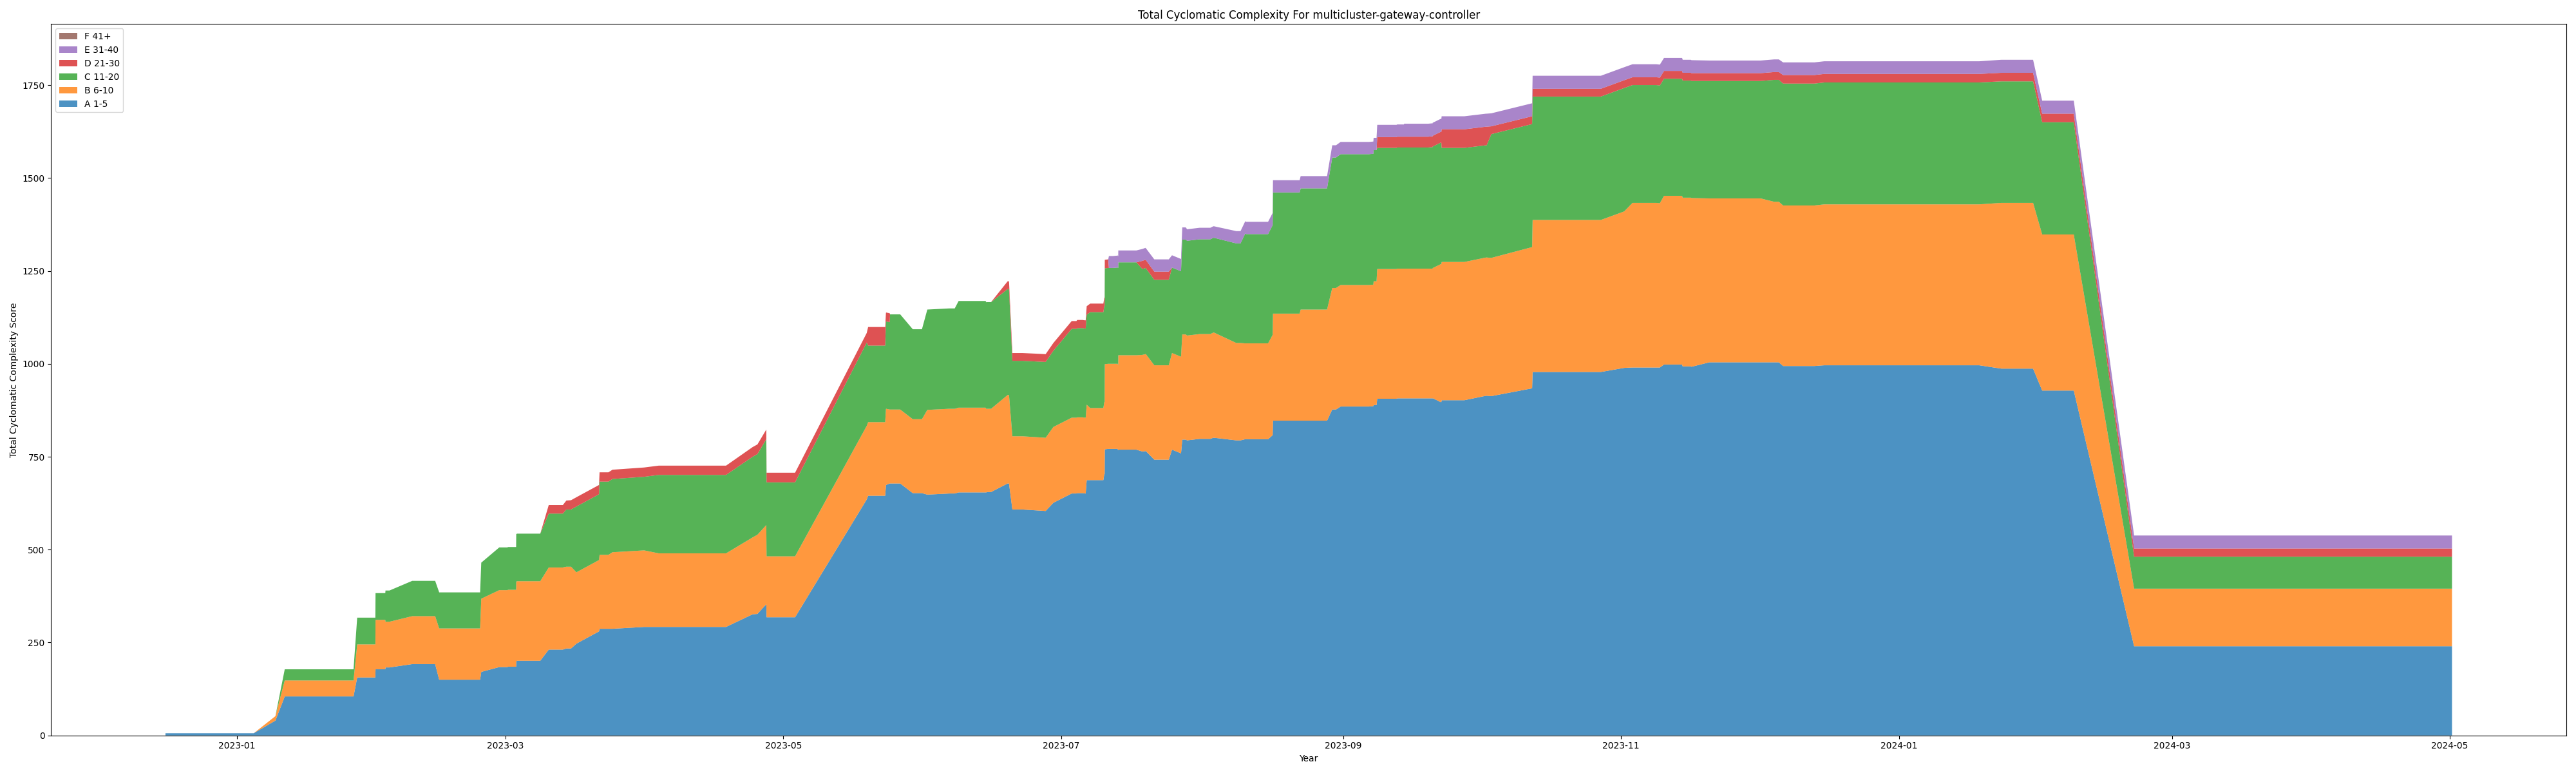
\includegraphics[width=\textwidth]{total_cc_mgc.png}
	\caption{Total \cc over time for multicluster-gateway-controller.}
	\label{fig:total_cc_mgc}
\end{figure}









